\documentclass[a4paper]{article}
\usepackage[french]{babel}
\usepackage{amsmath}
\usepackage{hyperref}
\usepackage{parskip}
\usepackage{graphicx}

\title{Équation d'une lentille mince}
\author{Prof. Yves Chevallier}
\date{\today}

\begin{document}
\maketitle
\begin{center}
    \textbf{Résumé}\par
\end{center}
    Cet article démontre l'équation d'une lentille mince dans sa première approximation.

\section{Introduction à l'environnement math}

\begin{figure}[h]
    \centering
    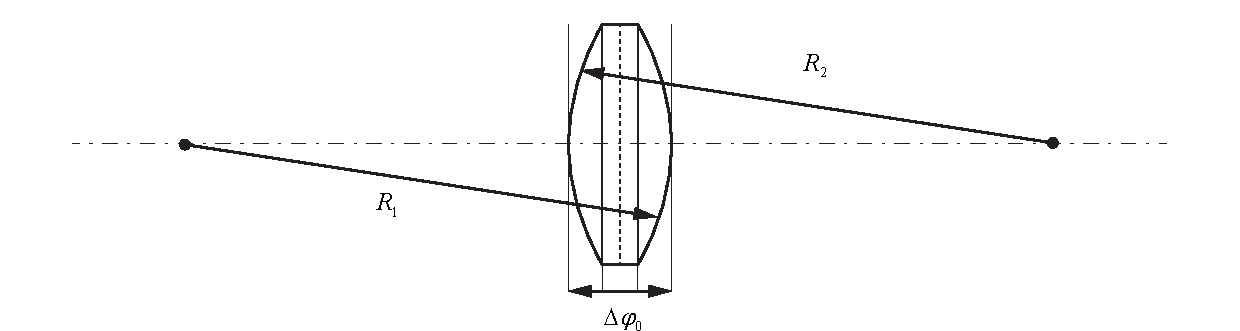
\includegraphics[width=\textwidth]{tlens.pdf}
    \caption{Une lentille biconvexe}
\end{figure}

Un arrangement 2-f est connu sous la dénomination de lentille de Fourier. On considère un verre bixonvexe d'une épaisseur $T$ d'un rayon de courbure $R_1$ et $R_2$ qui modifie spatialement la phase de la lumière incidente. Dans l'objectif d'obtenir l'équation générale \cite{goodman} qui sera utilisée plus tard, le délai de phase pour chaque position de la lentille peut être exprimé comme: 

\begin{equation}
    \Delta\varphi(x,y)=\Delta\varphi_0-R_1\left(1-\sqrt{1-\frac{x^2+y^2}{R_1^2}}\right)
    \label{eq:goodman}
\end{equation}

Où $\Delta\varphi_0$ correspond au déphasage total à la position $(0,0)$. Cette expression peut-être simplifiée si l'on se restreint à la portion des fronts d'ondes proches de l'axe horizontal de la lentille. Cette approximation et obtenue par les deux premiers termes d'une série de Taylor $\sqrt{1-x}$ évalué autour de $0$. En considérant l'approximation paraxiale, l'équation \ref{eq:goodman}

\begin{equation}
\Delta\varphi(x,y)\approx=\Delta\varphi_0-\frac{x^2+y^2}{2}\left(\frac{1}{R_1}-\frac{1}{R_2}\right)
\label{eq:toto}
\end{equation}

Enfin, cette transformation de phase peut être réécrite dans les termes suivants: 

\begin{equation}
\begin{split}
L(x,y) &= \exp\left(-i\frac{2\pi}{\lambda}(n\Delta\varphi(x,y)+\Delta\varphi_0-\Delta\varphi(x,y))\right) \\
       &= \exp\left(-i\frac{2\pi}{\lambda}\Delta\varphi_0\right) \exp\left(-i\frac{2\pi}{\lambda f}(n-1)\Delta\varphi(x,y)\right) \\
       &= \exp\left(-i\frac{2\pi}{\lambda}\Delta\varphi_0\right) \exp\left(-i\frac{2\pi}{\lambda f}(x^2+y^2)\right)       
\end{split}
\end{equation}

Les paramètres physiques peuvent être groupés en un paramètre nommé longueur focale. La constante du dépasage peut-être éliminée:

\begin{equation}
    \frac{1}{f}=(n-1)\left(\frac{1}{R_1}-\frac{1}{R_2}\right)
\end{equation}

Finalement, l'équation de la lentille mince est exprimée par:

\begin{equation}
    L(x,y)=\exp\left(-i\frac{2\pi}{\lambda}(x^2+y^2)\right)
\end{equation}

\begin{thebibliography}{1}
    \bibitem{goodman}
    Joseph W. Goodman, "The Optics of Thin Lens", Dover, New York, NY, 1964.
\end{thebibliography}
\end{document}